
\Chapter{INTRODUCTION}\label{sec:intro} \selectlanguage{english}

\section{Context and Motivation}

The research project is an EU-Canadian joint research project, which is called "EPICEA" - Electromagnetic Platform for
lightweight Integration/Installation of electrical systems in Composite Electrical Aircraft, will approach
numerous avionic engineering design issues in the advancement of future aircraft, aiming at a significant
reduction of energy consumption through more electrical aircraft and systems integration. This project strives to understand the electromagnetic (EM) issues on composite electric aircraft (CEA). This includes the analysis
and characterization of EM coupling, interconnects, and cosmic radiations (CR) on electrical systems together
with new concepts of antennas designed to maintain performance in composite environment without modifying
aircraft aerodynamics. Our contribution to this project --- "the study of CR effects on aircraft electrical systems." This research work will focus on design and implementation of the FPGA-based platform to help to investigate the effects of cosmic radiation (CR) on embedded electronic system of the aircraft. This project also aims to make the higher-level model that will use to investigate the effects of (CR) on the aircraft flying at the altitude of 40,000 feet. This project helps to find; at higher altitude when aircraft gets more exposure to the radiation; need a way to know early in the embedded electronic design of the aircraft if mitigation strategies are required to deal this higher radiation level. 

Space radiation has two preliminary sources --- galactic cosmic radiation and solar energetic particles~\cite{SWE20216}. Galactic cosmic radiation from outside the solar system consists mostly of energetic protons and heavy ions, e.g., iron. Solar energetic particles are commonly associated with the solar flare events and largely dominated by the proton. The consequences of these radiations on human health had been studied extensively at national and international levels. A global framework is also available for the addressing of these radiation issues on health particularly for the frequent flyer, e.g., air-crew. Most of the efforts done so far are either on the monitoring, modeling, and measurements of the radiation and improved the air-safety standards. The space radiation is an unavoidable space weather phenomena. The impact and consequences of the high-energy particles and thermalized neutrons on the avionics embedded system are now recognized as an area of active research. Especially, the incident happened with the Qantas Flight Airbus A330-303 flying from |Singapore to Perth went under the two terrifying dives due to the malfunction of the on-flight computer. After, the investigation it revealed that high-energy particles from the outer space --- were the responsible for the malfunction of the computer. And, the potential triggering event was the single-event effect (SEE) interacting with one of the integrated circuits (ICs) within the CPU module. 

Therefore, fault management strategies are essential to apply on the aircraft's embedded systems. In future, the FPGAs will replace the deterministic computer architecture platform provide more flexibility to flight operations. In FPGAs the configuration bits of the configuration memory that control the resources, user logic, routing resources, LUTs, CLBs, BRAM, DSP, and IOB blocks. If ion hits the FPGA, it can affect the memory resources that lead towards the fault, which may result in a failure. Before need to know to apply the mitigation techniques early in the embedded electronic design, we need to make the higher-level fault model of the systems that facilitate without going into the detailed simulation get the faulty behavior of the component at high-level.

  

\section{Problem Statement}

Cosmic rays are originating in outer space and travel at nearly the speed of light and strike the earth from all directions. These cosmic radiations are ranging from lightest to heaviest elements in the periodic table. When these high-energy cosmic rays interact with the earth's magnetosphere, neutrons are generated, often referred to as an air shower~\cite{lesea2005rosetta}. Neutron with energy greater than 10 MeV carries sufficient energy to cause single-event effects in SRAM-based FPGAs. An intense neutron environment exists at higher altitudes in the atmosphere, 10 km to 40 km.  Long-haul aircraft flying at the altitudes of 40,000 feet nearly 12 km at the latitude of \ang{60} as shown in Figure~\ref{fig:neu-flux}  under the influence of greatest neutron flux of all flights --- approximately 500 times that a ground-based observer in Newyork City~\cite{lesea2005rosetta}. This high-energy neutron passes through the silicon substrate of a device, and if the charge of these particles is sufficient enough to change the state of the configuration memory of the FPGA results in a drastic consequence. In this work, we will mainly focus on defining the pre-certification strategy that before employing the circuit in a robust condition, realistically evaluate the faulty behaviors of the circuit. The study of CR effects on aircraft at high altitude/latitude to be able to decide on the appropriate protection solution.


\begin{figure}
 \centering
  \captionsetup{justification=centering}    
   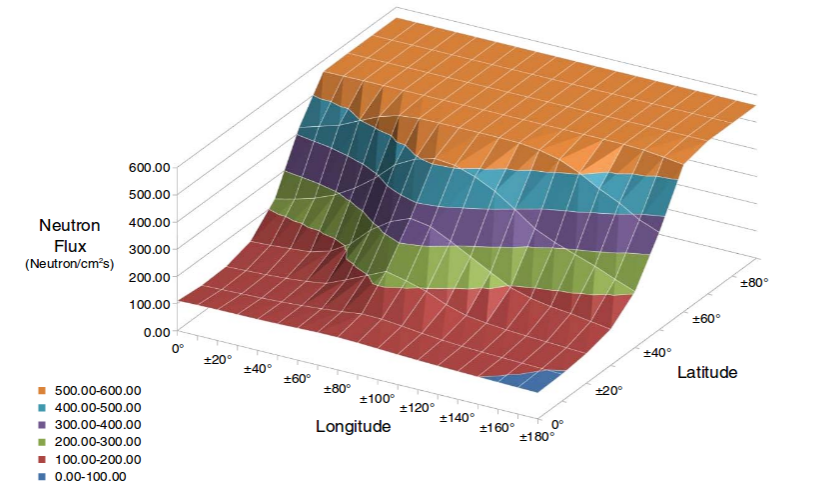
\includegraphics[scale=0.4]{figures/img/neutron-flux.png}
   \caption{Neutron Flux at 40,000 Feet.}
\label{fig:neu-flux}
\end{figure}





\section{Research Objectives}



The main objective of this project is to develop a faulty behaviour model for FPGA-based
circuits described at a high-level of abstraction.

By using neural networks, fault behaviour
models are developed and their accuracy is validated. The developed models could be used to
replace any component of the entire circuit with faulty versions of the components described
at a high-level of abstraction

The
goal of this research was to develop an approach for modeling the faulty behaviour of a
digital circuit in the presence of cosmic rays.

his ensures that the effect of faulty behaviour of each
component on a system could be analyzed at a high-level of abstraction and the mitigation
technique could be used to improve the robustness of more critical parts


The
goal of this research was to develop an approach for modeling the faulty behaviour of a
digital circuit in the presence of cosmic rays.


To implement effective high-level CR computer model one has to (a) design and implementation of the emulation system, (b) design and implementation of an experimental setup for bombardment,  c) feasible for aerospace system, and d) develop  a strategy to develop a high-level model from the results (signatures) derived from the emulation and bombardment setup. In the context of the development of a whole simulation methodology including CR environment and CR effects at
system and component levels, the objectives of this projects are:

\begin{itemize}
\item The goal of this work is to provide a fault injection platform flexible and optimized for
FPGA-based systems, allowing emulate configuration faults on SRAM-based FPGAs

\item Define CR environment in the context of future aircraft structures  at the level of electrical systems
\item Study existing databases of effects of CR at electrical systems level
\item Complete the analyses of the result of the CR characteristics recorded and derive the consequences in the aircraft embedded system
\item Develop the computer model of the CR effects
\item Simulate numerically the effect at component and electrical system level
\item Develop a strategy for evaluating the robustness of systems against CR
\item Propose update of CR requirements for electrical systems
\item Proposed the methodology and the models based on data observed in on-board experiments


\end{itemize}



The main challenges we foresee are:
\begin{itemize}
\item Development of the complex circuits and testing under radiation, e.g., soft-error analysis for sequential circuits
\item Make a model at higher-level of abstraction from the data extracted at lower level 
\item Experimental set-up for bombardment

\end{itemize}


  

\section{Novelty and Impact}


\begin{itemize}
\item The development and implementation of an early validation strategy at higher abstraction level helps to identify at what extent mitigation strategies are required
\item Study the system susceptibility under neutron-induced single even effect
\item Compare the neutron induced and proton induced errors
\item Signature for the sequential circuit
\item Computer model to study CR effects at early in the embedded system design
\end{itemize}


%%% Local Variables:
%%% mode: latex
%%% TeX-master: "../Document"
%%% End:
